\documentclass{beamer}

% Tema clássico
\usetheme{Madrid}
\usecolortheme{default}

% Pacotes essenciais
\usepackage[utf8]{inputenc}
\usepackage{graphicx}
\usepackage{booktabs}
\usepackage{amsmath}
\usepackage{amsfonts}
\usepackage{amssymb}
\usepackage{tikz}
\usepackage{pgfplots}
\pgfplotsset{compat=1.18}

% Informações da apresentação
\title{Apresentação de Teste}
\subtitle{Exemplo Completo em \LaTeX}
\author{Autor Exemplo}
\institute{Instituição Exemplo}
\date{\today}

\begin{document}

% Slide 1 - Capa
\begin{frame}
  \titlepage
\end{frame}

% Slide 2 - Sumário
\begin{frame}{Sumário}
  \tableofcontents
\end{frame}

% Slide 3 - Introdução
\section{Introdução}
\begin{frame}{Introdução}
  Esta é uma apresentação de teste criada em \LaTeX\ utilizando o pacote
  \textbf{Beamer}.  
  O objetivo é demonstrar diversos recursos comuns em apresentações acadêmicas.
\end{frame}

% Slide 4 - Texto e Parágrafo
\begin{frame}{Texto e Parágrafo}
  O \LaTeX\ é amplamente utilizado para produção de documentos científicos,
  pois oferece alta qualidade tipográfica e excelente controle de formatação.

  \vspace{0.5cm}

  Além disso, ele é especialmente indicado para documentos que contêm fórmulas
  matemáticas, tabelas e referências.
\end{frame}

% Slide 5 - Lista Simples
\begin{frame}{Lista Simples}
  \begin{itemize}
    \item Alta qualidade tipográfica
    \item Organização estrutural
    \item Facilidade com matemática
    \item Uso acadêmico e profissional
  \end{itemize}
\end{frame}

% Slide 6 - Lista Enumerada
\begin{frame}{Lista Enumerada}
  \begin{enumerate}
    \item Introdução
    \item Desenvolvimento
    \item Resultados
    \item Conclusão
  \end{enumerate}
\end{frame}

% Slide 7 - Fórmula Matemática Simples
\section{Matemática}
\begin{frame}{Fórmula Matemática}
  A famosa equação da relatividade é dada por:
  \[
    E = mc^2
  \]
  onde $E$ é a energia, $m$ a massa e $c$ a velocidade da luz.
\end{frame}

% Slide 8 - Fórmula Avançada
\begin{frame}{Equação Mais Elaborada}
  \[
    \int_{a}^{b} f(x)\,dx = F(b) - F(a)
  \]
  Essa equação representa o \textbf{Teorema Fundamental do Cálculo}.
\end{frame}

% Slide 9 - Bloco de Destaque
\begin{frame}{Bloco de Informação}
  \begin{block}{Definição}
    Uma função é uma relação que associa cada elemento de um conjunto
    a exatamente um elemento de outro conjunto.
  \end{block}
\end{frame}

% Slide 10 - Citação
\section{Citações}
\begin{frame}{Citação}
  \begin{quote}
    ``A matemática é a linguagem com a qual Deus escreveu o universo.''  
    \hfill — Galileu Galilei
  \end{quote}
\end{frame}

% Slide 11 - Tabela Simples
\section{Tabelas}
\begin{frame}{Tabela Simples}
  \begin{table}
    \centering
    \begin{tabular}{l c c}
      \toprule
      Item & Valor A & Valor B \\
      \midrule
      A & 10 & 20 \\
      B & 15 & 25 \\
      C & 30 & 40 \\
      \bottomrule
    \end{tabular}
    \caption{Exemplo de tabela}
  \end{table}
\end{frame}

% Slide 12 - Tabela Comparativa
\begin{frame}{Tabela Comparativa}
  \begin{tabular}{l c}
    \textbf{Tecnologia} & \textbf{Popularidade} \\
    \hline
    LaTeX & Alta \\
    Word & Muito Alta \\
    Markdown & Média \\
  \end{tabular}
\end{frame}

% Slide 13 - Gráfico de Barras
\section{Gráficos}
\begin{frame}{Gráfico de Barras}
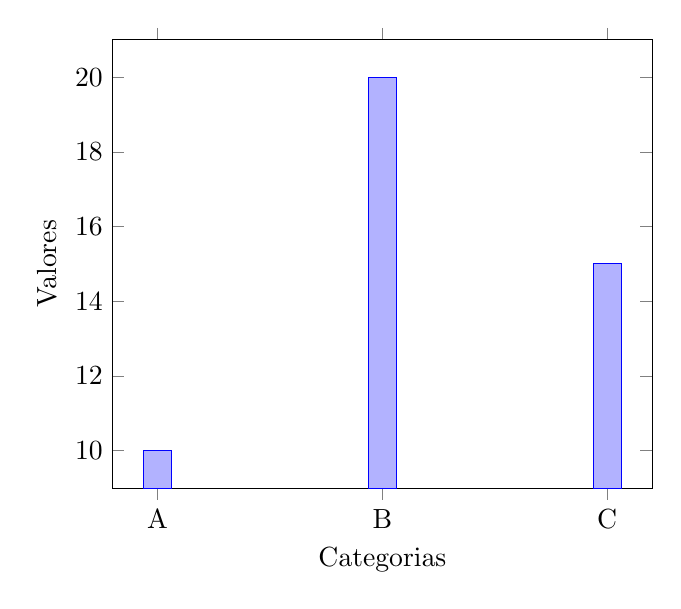
\begin{tikzpicture}
\begin{axis}[
    ybar,
    xlabel={Categorias},
    ylabel={Valores},
    symbolic x coords={A,B,C},
    xtick=data
]
\addplot coordinates {(A,10) (B,20) (C,15)};
\end{axis}
\end{tikzpicture}
\end{frame}

% Slide 14 - Gráfico de Linha
\begin{frame}{Gráfico de Linha}
\begin{tikzpicture}
\begin{axis}[
    xlabel={Tempo},
    ylabel={Crescimento}
]
\addplot coordinates {
    (1,2) (2,4) (3,6) (4,9)
};
\end{axis}
\end{tikzpicture}
\end{frame}

% Slide 15 - Texto + Fórmula
\section{Combinações}
\begin{frame}{Texto e Matemática}
  O crescimento exponencial pode ser modelado por:
  \[
    f(x) = a \cdot e^{bx}
  \]
  Esse tipo de função aparece em diversas áreas da ciência.
\end{frame}

% Slide 16 - Alerta
\begin{frame}{Alerta}
  \begin{alertblock}{Atenção}
    Sempre revise a estrutura e a coerência da sua apresentação.
  \end{alertblock}
\end{frame}

% Slide 17 - Exemplo Visual Simples
\section{Elementos Visuais}
\begin{frame}{Forma Geométrica}
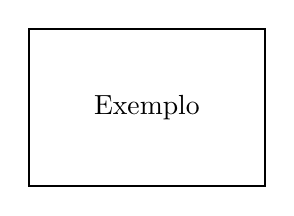
\begin{tikzpicture}
  \draw[thick] (0,0) rectangle (3,2);
  \draw (1.5,1) node {Exemplo};
\end{tikzpicture}
\end{frame}

% Slide 18 - Texto Final
\section{Conclusão}
\begin{frame}{Conclusão}
  O Beamer permite criar apresentações profissionais,
  organizadas e altamente personalizáveis.
\end{frame}

% Slide 19 - Considerações Finais
\begin{frame}{Considerações Finais}
  Esta apresentação demonstrou:
  \begin{itemize}
    \item Texto
    \item Tabelas
    \item Gráficos
    \item Fórmulas
  \end{itemize}
\end{frame}

% Slide 20 - Encerramento
\begin{frame}{Obrigado!}
  \centering
  \Large Perguntas?
\end{frame}

\end{document}
